% This is samplepaper.tex, a sample chapter demonstrating the
% LLNCS macro package for Springer Computer Science proceedings;
% Version 2.20 of 2017/10/04
%
\documentclass[runningheads]{llncs}
%
\usepackage{graphicx}
% Used for displaying a sample figure. If possible, figure files should
% be included in EPS format.
%
% If you use the hyperref package, please uncomment the following line
% to display URLs in blue roman font according to Springer's eBook style:
% \renewcommand\UrlFont{\color{blue}\rmfamily}
\usepackage{subcaption}
\captionsetup{compatibility=false}

\usepackage{floatrow} 
\usepackage[framemethod=tikz]{mdframed}
\usepackage{amsmath}
\usepackage{amsfonts}
\begin{document}
%
\title{Efficient creation of 3D organic models from sketches and ODE-based deformations}
%
\titlerunning{3D organic models from sketches and ODE-based deformations}
% If the paper title is too long for the running head, you can set
% an abbreviated paper title here
%
\author{Ouwen Li\inst{1} \and Shaojun Bian\inst{1} \and Algirdas Noreika\inst{2} \and Ismail Khalid Kazmi\inst{3} \and Lihua You\inst{1} \and Jianjun Zhang\inst{1}}
%
\authorrunning{Ouwen Li  et al.}
% First names are abbreviated in the running head.
% If there are more than two authors, 'et al.' is used.
%
\institute{National Centre for Computer Animation, Bournemouth University, Dorset, UK \\
Indeform Ltd., K. Petrausko g. 26, Kaunas 44156, Lithuania\\
 Teesside University, Middlesbrough, Tees Valley, UK }
%
\maketitle              % typeset the header of the contribution
%
\begin{abstract}
Efficient creation of 3D organic models is an important topic. In this paper, we propose a new approach to create rough 3D organic base models easily and quickly. The proposed approach first generates 2D sketches by manually drawing outlines of 3D organic objects or extracting outlines from 2D images. Then the generated outlines are decomposed into parts. For each of the decomposed parts, a central line is calculated from the two corresponding sketch segments. A straight cylinder is bent so that its central line coincides with the central line of the two corresponding sketch segments, and the radius of the cylinder is determined by minimizing the sum of the squared errors between the projected silhouette curves of the placed cylinder and the two corresponding sketch segments. Finally, an ordinary differential equation (ODE)-based and sketch-guided deformation algorithm is proposed to deform the cylinder so that the projected silhouette curves of the deformed cylinder exactly fit the two corresponding sketch segments. The experiment carried out in this paper  demonstrates that the approach proposed in this paper can create 3D organic base models from 2D sketches easily and quickly.


\keywords{3D organic base model creation  \and sketch generation \and automatic placements of 3D cylinders \and ODE-based deformations.}
\end{abstract}
%
%
%
\section{Introduction}
Polygon, NURBS and subdivision are three mainstream modelling approaches. They can create detailed and realistic 3D organic models and have been widely applied in various software packages such as Autodesk Maya and 3DS Max to carry out geometric modelling, computer graphics, computer animation and  computer-aided design applications etc. With these approaches, modellers usually import reference images from the concept artists, and then begin the modelling and sculpting operations. These reference images, sometimes called model sheets, are the profiles from T-pose or A-pose in front view, side view and back view respectively, or various arbitrary poses in arbitrary perspective views. Although these modelling approaches are very powerful and popular, they require great effort to learn how to use them, involve heavy manual operations, and take a lot of time to complete modelling tasks. \\

In order to address the above problems, various sketch-based modelling (SBM) approaches have been developed in the past several decades \cite{olsen2009sketch}. These approaches use the silhouettes of 3D objects to describe 3D models. According to Hoffman and Singh  \cite{hoffman1997salience}, for human vision systems, silhouettes alone are efficient for recognising everyday objects, by indexing their shapes in human memory. Also, we noticed that the most natural way for both novice modellers and veteran modellers to generate a new shape is to sketch freehand strokes with paper-pen-like graphic input tablets. So does the shape modification. In addition, the recent surge of painting or modelling applications in virtual reality such as Gravity Sketch \cite{GravitySketch}, Tilt Brush \cite{TiltBrush}, Quill \cite{Quill}, Medium \cite{OculusMedium} and Mozilla A-Painter \cite{APainter} also show artists have no problems in sketching in 3D canvas.\\

Once silhouettes of 3D objects are obtained, 3D models are created from these silhouettes. Although various sketch-based modelling approaches have been developed. All of them can be roughly divided into: direct shape generation, template-based mesh creation, and sketch-based deformation. Direct shape generation approaches are to create 3D models directly from 2D sketches. They can be further classified into: primitive-based 3D model creation and surface inflation. The approaches of template-based mesh creation deform a template 3D model to fit 2D sketches. Sketch-based Deformation methods use sketches to guide deformations of 3D models. Among these three different types of approaches, most research studies focus on creating 3D models directly from 2D sketches. The research study described in this paper belongs to this type. It quickly creates rough 3D models directly from 2D sketches. \\

Physics-based geometric modelling can greatly improve realism. Unfortunately, they usually involve heavy numerical calculations. Such a weakness makes physics-based geometric modelling less ideal for real-time 3D model creation. Ordinary differential equation (ODE)-based geometric modelling and shape deformations use the solution to a vector-valued ordinary differential equation to create 3D models and achieve shape deformations. Ordinary Differential Equations (ODE) have been widely used to describe various physical laws in scientific computing and engineering applications. For example, fourth-order ODEs have been used to describe the lateral bending of elastic beams in structural engineering. In this paper, we will use such a fourth-order ordinary differential equation to develop a new primitive deformation method.\\

A preliminary version of this work has been reported \cite{Li2019ODE}. It will first manually draw silhouette sketches of 3D organic objects or extract silhouette sketches from 2D images. Then the obtained silhouette sketches are decomposed into parts. For each of the decomposed parts, a central line is calculated from the two corresponding sketch segments. A straight cylinder is bent to make its central line coincide with the central line of the two corresponding sketch segments, and the radius of the cylinder is determined by minimizing the sum of the squared errors between the projected silhouette curves of the placed cylinder and the two corresponding sketch segments. Finally, an ordinary differential equation (ODE)-based and sketch-guided deformation algorithm is proposed to deform the placed cylinder so that the projected silhouette curves of the deformed cylinder exactly fit the two corresponding sketch segments. With the proposed approach, 3D organic base models are easily and quickly created.\\

The remaining parts of the paper will be structured below. First, the existing work will be reviewed in Section \ref{related work}. Next, manually drawing 2D sketches  and extracting the silhouette contours of 2D images will be discussed in Section \ref{Generation of 2d sketches}. After that, automatic placements of 3D cylinders guided by 2D sketches will be examined in Section \ref{Automatic placements of 3D primitives}. How to develop ODE-based and sketch-guided primitive deformations and fitting 3D cylinders to 2D sketches will be investigated in Section \ref{Fitting 3D primitives to 2D sketches}. Finally, conclusions will be drawn and future work will be discussed in Section \ref{Conclusion and future work}.

\section{Related work}\label{related work}
Sketch-based modelling and ODE-based geometric creation and shape deformations are two cornerstones. In this section, we review the existing work in these two fields.\\

\subsection{Sketch-based modelling}
Over the past several decades, sketch-based-modeling (SBM) has been widely studied in the computer graphic community \cite{olsen2009sketch}. It can be divided into: direct shape generation, template-based mesh creation, and sketch-based deformation. Direct shape generation can be further classified into: primitive-based 3D model creation and surface inflation.

\subsubsection{Direct shape generation} In the category of direct shape generation, several systems have been proposed to generate organic models. Here, we review two types of mesh: primitive-based 3D model creation and surface inflation.


\paragraph{Primitive-based 3D model creation}
An interesting phenomena is that many modeling system's building bricks are geometrical primitives of all sorts. In order to understand why geometrical primitives are chosen as the starting point of modelling a figure, we must first know how human vision system understands figures and interprets their shapes. \cite{hoffman1997salience} presented a theory of part salience. The theory builds on the minima rule for defining part boundaries. According to this rule, human vision defines part boundaries at negative minima of curvature on silhouettes, and along the negative minima of the principal curvatures on surfaces. They propose that the salience of a part depends on (at least) three factors: its size relative to the whole object, the degree to which it protrudes, and the strength of its boundaries. Based on this rule, a human character has many component parts which are often differ in their visual salience. For example, those sizes relative to the whole object are substantial, like torso; those protrude much from the main shape, like head, limbs and foot; and those have boundaries of sharp curvature changes, like neck.\\

The present evidence shows that these factors influence visual processes which determine the choice of figure and ground. Hence, we divide human figure into different parts based on these factors. Primitives-based systems decompose the modelling task as a process of creating a certain set of geometry primitives and further editing the primitives \cite{shtof2013geosemantic,chen2003visual,xu2016interactive}. The idea of assembling simple geometric primitives to form 3D models is very common in CSG (Constructive Solid Geometry) modelling. Shtof et al. \cite{shtof2013geosemantic} introduced a snapping method to detect the feature curves and silhouette curves of both 2D sketches and 3D simple geometric primitives, i.e. box, sphere, cylinder and cone, automatically determined the core parameters of these simple geometric primitives so as to fit the 2D sketches, and then improved the model globally by inferring geosemantic constraints that define the relationship between different parts, the relations including: parallelism, orthogonality, collinear centers, concentric, and coplanar. In the work of \cite{chen2003visual}, researchers proposed a tool to generate a cylinder from only 3 strokes: the first two strokes define the 2D profile and the last stroke defines the axis along which the profile curve sweeps. Copies of the profile are not only perpendicularly aligned to the axis, but also resized to snap to the input outlines. However, their work is only designed for man-made objects, where simple sweeping surfaces can meet the quality requirements of the modeling task. Structured annotations for 2D-to-3D modelling \cite{gingold2009structured}, on the other hand, focus on organic modelling. It used two sets of primitives. One is generalized cylinders, created by the input of a single open sketch stroke represented as a spline, and then modified them by using simple gestures such as tilting cross sections, scaling local radius, rotating symmetrical plane, and changing cap size. The other primitives are ellipsoids, generated according to the drawn closed ellipse sketch strokes. As its name indicates, there exist a set of annotation tools to further edit the surface shape using annotations such as same lengths, same angles, alignments, and mirror symmetries. Its main contribution is providing a solution to the problem of semantic information such as symmetric, equal length and angle, and alignment, which are quite obscure in single view modelling system with only one arbitrary angled guide image. \\

\paragraph{Surface inflation} Another way to generate a shape is inflating a surface represented by closed 2D region/sketch to give it a volume \cite{kazmi2014survey}. The surface inflation technique extrudes a polygonal mesh from a given skeleton outwards and does a good job in modelling stuffed toys. One trend is to inflate freeform surfaces to create simple stuffed animals and other rotund objects in a SBM fashion \cite{igarashi2005rigid,nealen2007fibermesh,Karpenko:2006:SFS:1141911.1141928}. The pioneering Teddy system \cite{igarashi2005rigid} takes closed curves as inputs, finds their chordal axes as the spines, then wraps the spines with a polygonal mesh. Later, \cite{nealen2007fibermesh} enriches editing operations for the inflated base mesh. This approach also presents two types of the control curves: smooth and sharp. A smooth curve constrains the surface to be smooth across it, while a sharp curve only places positional constraints with $C^{0}$ continuity. Sharp control curves appear when operations like cutting, extrusion, and tunnel take place. They also serve the creation of creases on the surface. The Smooth Sketch system \cite{Karpenko:2006:SFS:1141911.1141928} supports the creation of cusps and T-junctions, which Teddy and its successors fail to address. In addition, SmoothSketch \cite{Karpenko:2006:SFS:1141911.1141928} extended Teddy’s work \cite{igarashi2005rigid} to an extent that the strokes do not need to be closed. Although the surface inflation approach is good at creating stuffed animals and simple toys, it is not versatile enough to express geometrical details on the surface. BendSketch \cite{li2017bendsketch} offers a technique which enables complex curvature patterns existing on surfaces. In order to give the bending information, users need to draw a set of lines that comply with what the BendSketch system \cite{li2017bendsketch} has specified, which mimics the hatching technique artists often utilise to express the sense of volume and curvature information on the surfaces.

\subsubsection{Template-based mesh creation} Using geometric primitives to align 2D sketches provides an easy and efficient approach to generate rough base models. However, manipulating the generated rough base models in one image plane only is difficult to create detailed 3D models. For template-based mesh creation, an elegant technique for sketch-based modeling has been proposed in \cite{kraevoy2009modeling} to find precise correspondences and determine mesh deformations. By combining skeleton-based deformation and mesh editing, an efficient approach was proposed in \cite{kazmi2015efficient} to quickly deform a 3D template model to fit the user’s drawn sketches. Among various approaches of direct shape generation from user-drawn sketches, a variety of sketch-based modelling tools are based on a “sketch-rotate-sketch" workflow. Such a workflow requires users to draw sketches from many views, causing the difficulties in matching input strokes with a guidance image and finding a good view \cite{gingold2009structured}.

\subsubsection{Sketch-based deformation}Deformation tools provide the interface for users to interact and modify the mesh surface. A good deformation tool should meet the following principles \cite{botsch2008linear}:
\begin{itemize}
    \item Flexibility: permit users to change the mesh surface as they wish, meanwhile reserve correct modelling constraints.
    \item Shape quality: aesthetically pleasing
    \item Intuitive result: conform to the morphing happen in real world with real physical material, which makes no recognition confusion for users when they modify the shape. In other words, physically correct.
\end{itemize}

Sketch-based shape editing like Teddy and others \cite{igarashi2005rigid,nealen2007fibermesh,Karpenko:2006:SFS:1141911.1141928} featured inflation approaches use smooth silhouettes. Therefore, they create only smooth shapes. In order to create aesthetically pleasing details on meshes, SBM should be equipped with shape editing method supporting inserting feature curves while preserve the global and local geometry. Geometry-based editing system is based on the energy in a form of geometrical traits. A popular geometry-based frame is Laplacian/Poisson model, which represents the differential traits of the surface in various ways depending on how they are employed. In the discrete Laplacian/Poisson models, it is easy to displace a set of edges (e.g., sketch a new position of an identified contour) while preserving the geometric details of the surface as much as possible \cite{nealen2007sketch}. In order to address the problem that feature lines’ differential properties are related to the viewing direction, and the feature lines do not coincide with edges on the mesh, \cite{nealen2007fibermesh} extends the framework of Laplace/Poisson mesh modelling in 3 ways: (a) accommodate constraints on the normals and the curvature; (b) allow constraints to be placed on virtual vertices, i.e. vertices placed on edges that only serve to implement the constraints but are never added to the mesh. The virtual vertices are linearly interpolated on the edge between 2 vertices; (c) incorporate a tangential mesh regularization, which moves edges onto sharp features while ensuring well-shaped triangles. Their method supports to change the moderate noisy silhouette contours, to edit the sharp feature lines like ridge, ravine and crease, and to edit smooth features and suggestive contours. Apart from deformation based on differential surface representations, another family makes use of multi-resolution or subdivision editing as a way to perform global surface deformation while preserve local surface details. Subdivision mesh is firstly decomposed into a low-frequency base surface and a high-frequency detail information. After deforming the base surface, the detail information is added to the deformed base surface. In the case of interactive shape editing by means of manipulating control handles with 3 degrees of freedom for translation and 3 degrees of freedom for rotation, the displacement vector is defined as the change of position and orientation of the control handles. The final shape can be seen as the outcome of adding a basis function of displacement vector to the origin shape. The requested displacement has to be translated into coefficients of this basis functions. These coefficients include but not limited to smoothness, stiffness (order of energy function), fullness, etc. Besides, the basis functions require pre-computed inverse matrix to speed up the surface updating \cite{botsch2004intuitive}, which is another hint that these approaches are very computational-expensive.  \cite{nealen2007sketch} proposed a sketch-based mesh editing system that can deform a user selected ROI (region of interest) to fit the input sketch. \cite{Zimmermann:2008:SIS:1411846.1411916} is able to compute from the oversketched feature line alone. 

\subsection{ODE-based geometric creation and shape deformations}
Compared to the geometry-based technology, physic-based editing technology simulates the physical principle through physical energy function. It complies with the real-world physical fidelity. However, it is less flexible if the 3D artists want to achieve very drastic effects because the penalty of stretching or bending forces on the energy function will be very big. Another challenge of physically based skin deformation methods is that they are computational-expensive, at least they are not as efficient as geometry based approaches. Hence, our object is to improve the performance and efficiency of physical-based editing scheme by decreasing the 2-dimensional partial differential equation to 1-dimensional ordinary differential equation. The finite element method and the finite difference method are widely used to solve various partial differential equations in this scenario. In this paper, we choose the finite difference method to solve the converted ordinary differential equation (ODE). \\ 
ODEs have been widely applied in scientific computing and engineering analyses to describe the underlying physics. For example, fourth-order ODEs have been used to describe the lateral bending deformations of elastic beams. Introducing ODEs into geometric processing can create physically realistic appearances and deformations of 3D models. ODE-based sweeping surfaces \cite{you2007boundary}, ODE-based surface deformations \cite{you2010shape,chaudhry2013shape}, and ODE-based surface blending \cite{you2014blending} have also been developed previously. 
Although researchers studied ODE-based geometric surface creation and deformations, how to use ODE-based modelling to deform geometric primitives and create new shapes from the user's drawn sketches has been under-explored to date. \\


\section{Generation of 2D sketches}\label{Generation of 2d sketches}
The first step of our proposed approach is to generate 2D sketches. Two methods are included in our developed system to generate 2D images. They are manually drawing without a reference image and extracting a 2D sketch from a reference image.\\

As investigated by Wuhrer and Shu \cite{Wuhrer2012Shape}, three different types of sketches can be drawn by users. These three types of sketches are: silhouette contours, occluding contours, and suggestive contours (Figure 1). Since this paper aims to develop a simple, easy, and efficient approach to create base 3D organic models from 2D sketches, we focus on silhouette contours only.\\

\begin{figure}
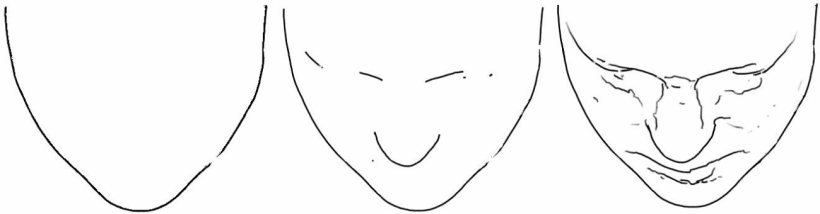
\includegraphics[width=\textwidth]{6233147-fig-1-source-large.png}
\caption{Three types of sketches: (a) silhouette contour, (b) occluding contour, and (c) suggestive contour of a face model. (Image source: Wuhrer and Wu \cite{Wuhrer2012Shape}).} 
\end{figure}

Our developed system allows users to draw the silhouette contours as shown in Figure \ref{fig:user draw}. If a reference image such as the one give in Figure \ref{fig:input 2d image} is available, our developed system allows users to trace the silhouette contours of the input image and obtain the silhouette contours of the input image as shown in Figure \ref{fig:extracted silhouette}.\\
\begin{figure}[!htbp]
    \centering
    \begin{subfigure}[b]{.4\columnwidth}
    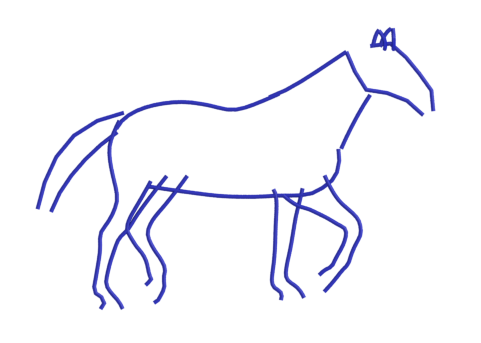
\includegraphics[height=1.6 in]{horse_silhouette.png}
    \caption{}
    \label{fig:user draw}
    \end{subfigure}
    \hspace{2em}
    \begin{subfigure}[b]{.2\columnwidth}
    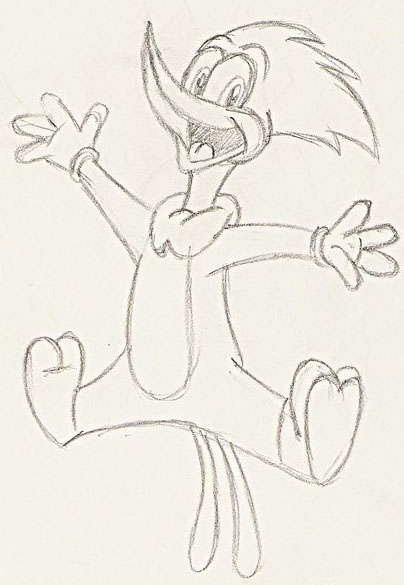
\includegraphics[height=1.6 in]{woody-woodpecker-sketch-16.jpg}
    \caption{}
    \label{fig:input 2d image}
    \end{subfigure}
    \hspace{2em}
    \begin{subfigure}[b]{.2\columnwidth}
    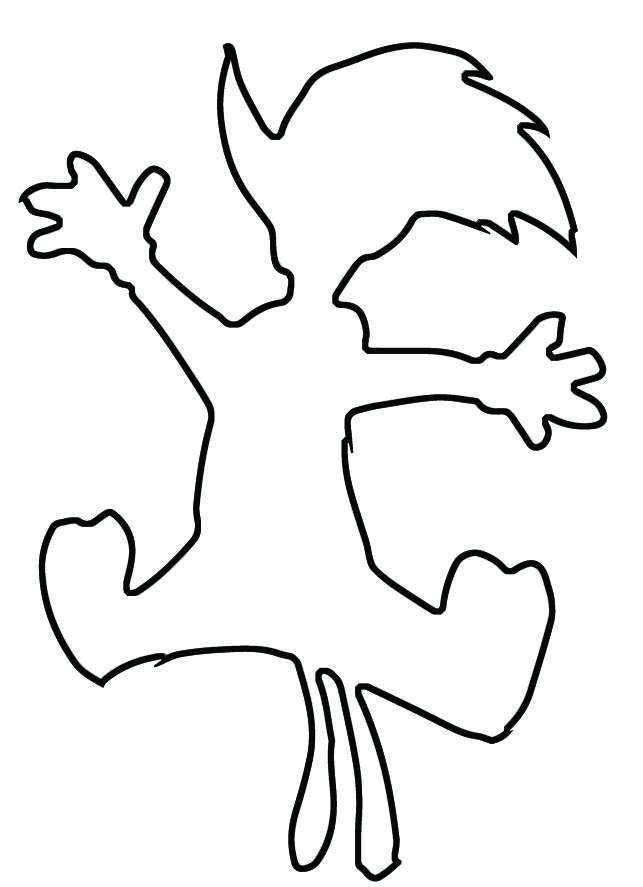
\includegraphics[height=1.6 in]{extracted_silhouette_from_sketch.jpg}
    \caption{}
    \label{fig:extracted silhouette}
    \end{subfigure}
    \caption{Generation of silhouette contours: (a) User-drawn silhouette contour, (b) input 2D image, (c) silhouette contour generated from the input 2D image}
    \label{fig:different means to input silhouette}
\end{figure}

\section{Automatic placements of 3D primitives}\label{Automatic placements of 3D primitives}
The second step of our proposed approach is to select suitable 3D primitives and automatically place the 3D primitives to best fit the user-generated 2D sketches. It involves: decomposing a 2D sketch into parts with each part defined by a closed or open sketch segment or two open sketch segments, calculating the central line of each part, initially placing a primitive along the central line, projecting the 3D primitive to obtain one or two silhouette contours, and scaling the size of the placed 3D primitive to minimize the error between the silhouette contours of the placed 3D primitive and the sketch segments of the decomposed part as elaborated below.\\

For a female sketch shown in Figure \ref{fig:dancer sketch}, 11 parts are decomposed. The 11 decomposed parts are 1 head, 1 neck, 2 hands, 2 arms, 1 torso, 2 legs, and 2 feet. Among them, the head is a closed sketch segment, each of 2 hands and 2 feet is an open sketch segment, and all other parts are defined by two open sketch segments.\\

The study carried out in \cite{Kazmi2016A} combines three 3D primitives to create rough 3D models. The three 3D primitives are: generalized cylinders, ellipsoids, and cubes. Organic objects have no sharp edges. Cubes may not be suitable in representing organic models. Although generalized cylinders are powerful in mathematically representing various cylinder-like shapes, they are difficult to operate in practice since the mathematical equation defining a generalized cylinder involves a variable and all the parameters defining the shape and size of a generalized cylinder are dependent on the variable. \\

\begin{figure}[htbp]
    \centering
    \begin{subfigure}{.2\columnwidth}
    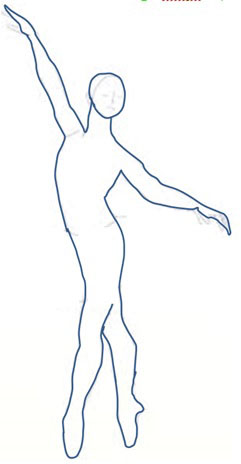
\includegraphics[height=1.4 in]{Fig3a.jpg}
    \caption{}
    \label{fig:dancer sketch}
    \end{subfigure}
    \begin{subfigure}{.2\columnwidth}
    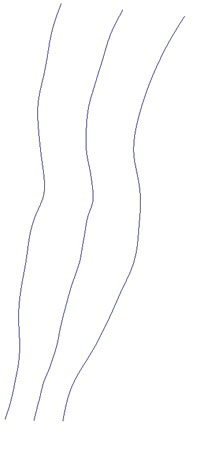
\includegraphics[height=1.4 in]{Fig3b.jpg}
    \caption{}
    \label{fig:leg silhouette}
    \end{subfigure}
    \begin{subfigure}[h]{.2\columnwidth}
    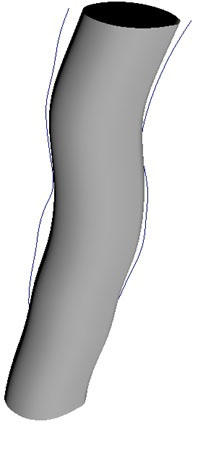
\includegraphics[height=1.4 in]{Fig3c.jpg}
    \caption{}
    \label{fig:leg bent}
    \end{subfigure}
    \begin{subfigure}{.2\columnwidth}
    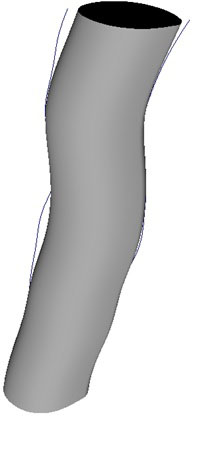
\includegraphics[height=1.4 in]{Fig3d.jpg}
    \caption{}
    \label{fig:leg bent with new radius}
    \end{subfigure}

    \begin{subfigure}{1.\columnwidth}
    \centering
    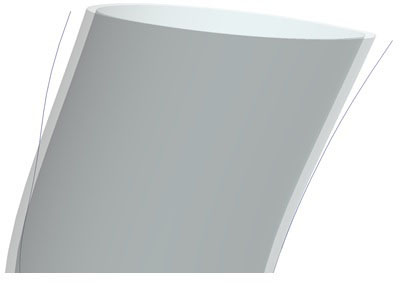
\includegraphics[height=2. in]{Fig3e.jpg}
    \caption{}
    \label{fig:cyliders comparison}
    \end{subfigure}
    \caption{Process of automatically placing curved cylinder}
    \label{fig:place curved cylinder}
\end{figure}

Based on the above discussions, this paper uses standard cylinders and ellipsoids as 3D primitives to represent 3D models. For ellipsoids, we scale them to best fit the 2D sketches like the female head which looks like an ellipse. For standard cylinders, we propose an ordinary differential equation (ODE)-based and sketch-guided deformation algorithm to change standard cylinders into various shapes to better approximate complicated 3D models. In what follows, we take the left leg of the female sketch to demonstrate how to automatically place a cylinder to fit the sketch segments of the left leg.\\

As shown in Figure \ref{fig:leg silhouette}, the left leg is defined by a left sketch segment and a right sketch segment. In order to place a 3D cylinder to best align with the sketch segments, we first determine the central line of the left leg. There are different methods which can be used to determine a central line of two sketch segments.  For example, we can generate a straight line from one starting point on one sketch segment and perpendicular to the sketch segment, find the intersecting point between the straight line and the other sketch segment, and use the middle point between the starting point and the intersecting point to create the central line. Here, we use the method below to generate central lines.\\

The total points on the left sketch segment may not be the same as the total points of the right sketch segment. From the points on each of the two sketch segments, we can calculate the total length of each of the two sketch segments. If we want to use N+1 points to define the central line, we divide each of the two total lengths by N to obtain N+1 points on each of the two sketch segments. That is to say, $P_{1,n}$ (n=1, 2, 3,…, N+1) points on the left sketch segment, and $P_{2,n}$ (n=1, 2, 3,…, N+1) points on the right sketch segment. The central line between the left sketch segment and the right sketch segment is generated from the points (n=1, 2, 3,…, N+1) determined by the equation below
\begin{equation}
\begin{split}
    C_n=P_{1,n}+0.5(P_{2,n}-P_{1,n})\\
    (n=1, 2, 3,…, N+1)   
\end{split}
\end{equation}
By connecting all the points $C_n$ together, we obtain the central line between the left sketch segment and the right sketch segment. The middle line shown in Figure \ref{fig:leg silhouette} gives the central line of the two sketch segments.\\

Next, we place a 3D cylinder to align with the two sketch segments. Since the central line is not straight, if straight cylinders without bending are chosen as 3D primitives, at least two or more cylinders have to be used and the space between two disconnected cylinders must be blended together to create the 3D left leg model. Clearly, this method of creating the 3D leg model is not a good choice. In this paper, we propose another method. With this method, a straight cylinder is bent by the central line. That is to say, the central line of the bent cylinder is the same as the central line between the two sketch segments. The radius of the bent cylinder is determined by the following equation
\begin{equation}
    r=\frac{1}{N+1}\sum_{n=1}^{N+1}\left\|P_{2,n}-P_{1,n}\right\|/2
    \label{radius average}
\end{equation}

For the leg shown in Figure \ref{fig:leg silhouette}, we obtain $r=0.537$ from Eq. \eqref{radius average}. With the obtained radius, a straight cylinder is bent and placed along the central line. The obtained bent cylinder is shown in Figure \ref{fig:leg bent}. \\
The radius of the bent cylinder determined above is not optimal. It can be improved by minimizing the total error between the two projected silhouette curves of the bent cylinder and the two sketch segments. Similar to the above treatment, after projecting the bent cylinder to the plane of the two sketch segments, we obtain two projected silhouette curves. Then we draw straight lines passing through the points $P_{1,n}$, $C_n$, and $P_{2,n}$, and calculate the intersecting points between the straight line and the two projected silhouette curves to obtain the N+1 points $C_{1,n}$ on the left projected silhouette curve and N+1 points $C_{2,n}$ on the right projected silhouette curve. If the radius of the bent cylinder is changed from $r$ to $\bar{r}$, the left projected silhouette curve will be changed from $C_{1,n}$ to $\bar{C}_{1,n}$, and the right projected silhouette curve will be changed from $C_{2,n}$ to $\bar{C}_{2,n}$ where $\bar{C}_{1,n}$ and $\bar{C}_{2,n}$ are determined by the equations below
\begin{equation}
    \begin{split}
        \Bar{C}_{1,n}=C_n-\frac{\Bar{r}}{r}(C_n-C_{1,n}) \\
        \Bar{C}_{2,n}=C_n+\frac{\Bar{r}}{r}(C_{2,n}-C_n) \\
        (n=1,2,\ldots,N+1)
    \end{split}
    \label{projected silhouette}
\end{equation}
The optimal radius $\bar{r}$ of the bent cylinder can be obtained by minimizing the sum of the squared errors between two new projected silhouette curves and the two sketch segments, i. e., 
\begin{equation}
    \min_{\bar{r}}\sum_{n=1}^{N+1}\|\bar{C}_{1,n}-P_{1,n}\|+\|\bar{C}_{2,n}-P_{2,n}\|
    \label{optimal radius}
\end{equation}

Introducing Eq.\eqref{projected silhouette} into Eq. \eqref{optimal radius}, Eq.\eqref{optimal radius} is changed into
\begin{equation}
    \min_{\Bar{r}}\sum_{n=1}^{N+1}\|C_n-\frac{\bar{r}}{r}(C_n-C_{1,n})-P_{1,n}\|+\|C_n+\frac{\bar{r}}{r}(C_{2,n}-C_n)-P_{2,n}\|
    \label{optimal radius expand}
\end{equation}

Solving the minimization equation \eqref{optimal radius expand}, we obtain the optimal radius $r=0.574$. Using the value, we generate a new bent cylinder shown in Figure \ref{fig:leg bent with new radius} whose radius makes the two projected silhouette curves better approximate the two sketch segments. Figure \ref{fig:cyliders comparison} gives a comparison of the cylinders whose radii are determined by Eqs. \eqref{radius average} and \eqref{optimal radius expand}, respectively. 

\section{Fitting 3D primitives to 2D sketches}\label{Fitting 3D primitives to 2D sketches}
The last step of our proposed approach is to develop an ordinary differential equation-based and sketch-guided deformation algorithm and use the algorithm to deform the placed cylinders so that the projected silhouette curves of the deformed cylinders exactly fit the two sketch segments of the decomposed parts. In what follows, we will elaborate how to develop such an ODE-based and sketch-guided deformation algorithm from a simplified version of the Euler-Lagrange PDE (Partial Differential Equation), which is widely used in physically-based surface deformations and briefly reviewed below.\\
As discussed in \cite{botsch2008linear}, the main requirement for physically-based surface deformations is an elastic energy which considers the local stretching and bending of two-manifold surfaces called thin-shells. When a surface $S \subset R^3$, parameterized by a function $P(u, v): \omega \subset R^2 \mapsto S \subset R^3$, is deformed to a new shape $S'$ through adding a displacement vector $\textbf{d}(u, v)$ to each point $\textbf{P}(u, v)$, the change of the first and second fundamental $\textbf{I}(u, v)$, $\textbf{II}(u, v) \in R^{2 \times 2}$ forms in differential geometry \cite{do2017differential} yields a measure of stretching and bending, as described in \cite{terzopoulos1987elastically}:

\begin{equation}
    E_{shell}(\mathbb{S'}) = \int_{\Omega}k_s\|I'-I\|_F^2+k_b\|\Pi'-\Pi\|_F^2 dudv  
\label{energy}
\end{equation}

where $\textbf{I}\;'$ and $\textbf{II}\;'$ are the first and second fundamental forms of the surface $S\;'$, $\parallel . \parallel$  indicates a (weighted) Frobenius norm, and the stiffness parameters $k_{s}$ and $k_{b}$ are used to control the resistance to stretching and bending.

Generating a new deformed surface requires the minimization of the above Equation \eqref{energy}, which is non-linear and computationally expensive for interactive applications. In order to avoid the nonlinear minimization, the change of the first and second fundamental forms is replaced by the first and second order partial derivatives of the displacement function $\textbf{d}(u, v)$ \cite{celniker1991deformable,welch1992variational}, i. e.,

\begin{equation}
    \tilde{E}_{shell}(\mathbf{d})=\int_{\Omega}k_s(\|\mathbf{d}_u\|^2+\|\mathbf{d}_v\|^2)+k_b(\|\mathbf{d}_{uu}\|^2+2\|\mathbf{d}_{uv}\|^2+\|\mathbf{d}_{vv}\|^2) dudv
    \label{energydiffgeo}  
\end{equation}

where $ d_{x}=\frac{\partial}{\partial x}d$ , $d_{xy}=\frac{\partial}{\partial x \partial y }d$ and $d_{xx}=\frac{\partial}{\partial {x^2}}d$. 
The minimization of the above equation can be obtained by applying variational calculus, which leads to the following Euler-Lagrange PDE:

\begin{equation}
     -k_s\triangle \mathbf{d}+k_b\triangle^2\mathbf{d}=0,    
    \label{lagrange}     
\end{equation}

where $\triangle$ and $\triangle ^ {2}$ are the Laplacian and the bi-Laplacian operators, respectively,

\begin{equation}
\begin{split}
    \triangle \mathbf{d}=div\nabla \mathbf{d}=\mathbf{d}_{uu}+\mathbf{d}_{vv}, \\  \triangle^2\mathbf{d}=\triangle(\triangle \mathbf{d}) =\mathbf{d}_{uuuu}+2\mathbf{d}_{uuvv}+\mathbf{d}_{vvvv}.
\end{split}
\label{laplacianoperator}   
\end{equation}

Using the sketched 2D silhouette contours shown in Fig. \ref{fig:leg silhouette} to change the shape of the cylinder can be transformed into the generation of a sweeping surface which passes through the two sketched 2D silhouette contours. The generator that creates the sweeping surface is a curve of the parametric variable $u$ only, and the two silhouette contours are trajectories. If Equation \eqref{lagrange} is used to describe the generator, the parametric variable $v$ in Equation \eqref{lagrange} drops, and we have $d_{vv} = 0$ and $d_{vvvv} = 0$. Substituting $d_{vv} = 0$ and $d_{vvvv} = 0$ into Equation \eqref{laplacianoperator}, we obtain the following simplified version of the Euler-Lagrange PDE, seen as \eqref{ODE}, which is actually a vector-valued ODE.
\begin{equation}
k_b\frac{\partial^4\mathbf{d}}{\partial u^4}-k_s\frac{\partial^2 \mathbf{d}}{\partial u^2}=0.
\label{ODE}    
\end{equation}

As pointed out in \cite{chaudhry2013shape}, the finite difference solution to ODEs is very efficient, we here investigate such a numerical solution to Equation \eqref{ODE}. For a typical node $i$, the central finite difference approximations of the second and fourth order derivatives can be written as:

\begin{equation}
\begin{split}
    \frac{\partial^2\mathbf{d}}{\partial u^2}|_i =\frac{1}{\triangle u^2}(\mathbf{d}_{i+1}-2\mathbf{d}_i+\mathbf{d}_{i-1}), \\
    \frac{\partial^4\mathbf{d}}{\partial u^4}|_i =\frac{1}{\triangle u^4}[6\mathbf{d}_i-4(\mathbf{d}_{i-1}+\mathbf{d}_{i+1})+\mathbf{d}_{i-2}+\mathbf{d}_{i+2}].
\label{FDM}
\end{split}    
\end{equation}

Introducing Equation \eqref{FDM} into Equation \eqref{ODE}, the following finite difference equation at a representative node $i$ can be written as:
\begin{equation}
    \begin{split}
    (6k_b+2k_sh^2)\mathbf{d}_i+k_b\mathbf{d}_{i-2}+k_b\mathbf{d}_{i+2}-(4k_b+k_sh^2)\mathbf{d}_{i-1}-(4k_b+k_sh^2)\mathbf{d}_{i+1}=0.
    \label{odefdm}
    \end{split}    
\end{equation}

For organic models, the 3D shape defined by two silhouette contours is closed in the parametric direction $u$ as indicated in Fig. \ref{fig:finite node top view}. Therefore, we can extract some closed curves each of which passes through the two corresponding points on the two silhouette contours. Taking the silhouette contours in Fig. \ref{fig:finite node top view} as an example, we find two corresponding points $C_{13}$ and $C_{23}$ on the original silhouette contours $c_{1}$ and $c_{2}$, and two corresponding points $C'_{13}$  and $C'_{23}$ on the deformed silhouette contours $c'_{1}$ and $c'_{1}$ as shown in Fig. \ref{fig:finite node side view}. Then, we extract a closed curve $c(u)$ passing  through the two corresponding  points $C_{13}$  and $C_{23}$ from the 3D model in Fig. \ref{fig:finite node side view} and depict it as a dashed curve in Fig. \ref{fig:finite node top view}. Assuming that the deformed shape of the closed curve $c(u)$ is $c'(u)$, the displacement difference between the original closed curve and the deformed closed curve is $d(u) = c'(u)-c(u)$.

\begin{figure}[!htbp]
    \centering
    \begin{subfigure}[b]{.45\columnwidth}
    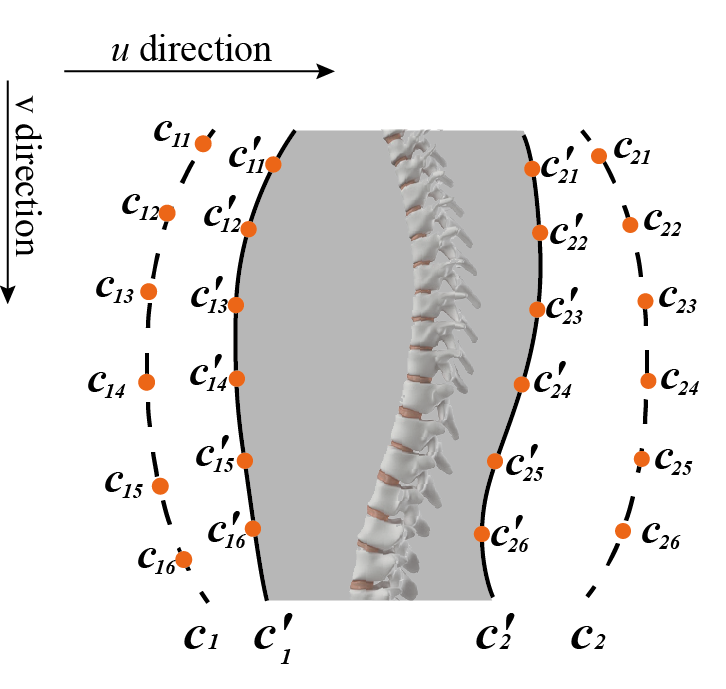
\includegraphics[height=2 in]{fdmnode_a.png}
    \caption{}
    \label{fig:finite node side view}
    \end{subfigure}
    \hspace{2em}
    \begin{subfigure}[b]{.45\columnwidth}
    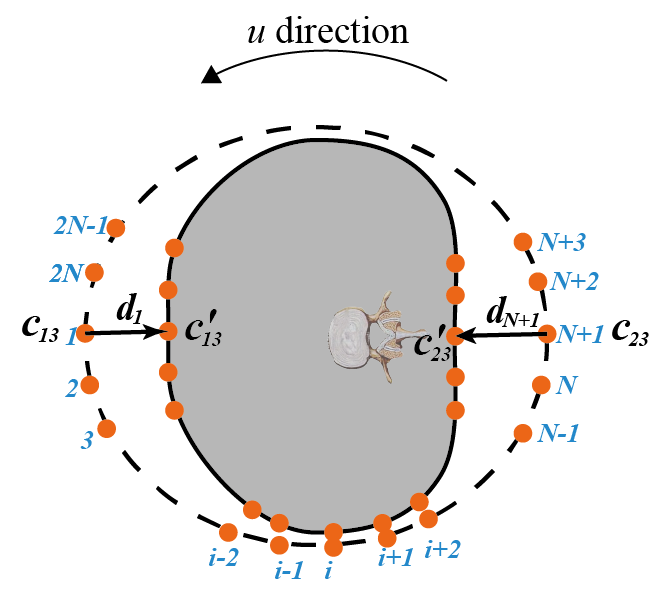
\includegraphics[height=2 in]{fdmnode_b.png}
    \caption{}
    \label{fig:finite node top view}
    \end{subfigure}
    \caption{Finite difference nodes for local shape manipulation from sketches in top and side view planes, respectively}
    \label{fig:different means to input silhouette}
\end{figure}

In order to use the finite difference method to find the displacement difference $d(u)$, we uniformly divide the closed curve into 2$N$ equal intervals as indicated in Fig. \ref{fig:finite node top view}. With the displacement difference at node 0 and node $N$ already known, i. e. $d_{0}=C'_{13}-C_{13}$ and $d_{N}=C'_{23}-C_{23}$, we can form a 2$N$ linear algebra equations derived from (12) for each of these nodes’ displacement. Solve the equations and add all the displacement differences to the original curve $c(u)$, we can then obtain the deformed curve $c'(u)$, and depict it as a solid curve in Fig. \ref{fig:finite node top view}. Repeating the above operations for all other points on the two silhouette contours, we obtain all deformed curves that describe a new 3D deformed shape. This method also applies to deformations responding to free form curves, which can be seen from the creation of a star model depicted in Fig. \ref{fig:sea star} and a human leg shown in Fig. \ref{fig:leg deformed twice}.

\begin{figure}[!htbp]
    \centering
    \begin{subfigure}[h]{.45\textwidth}
    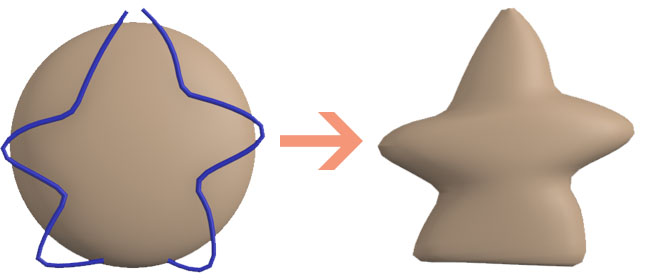
\includegraphics[height=1 in]{jelly.jpg}
    \caption{}
    \label{fig:sea star}
    \end{subfigure}
    \hspace{2em}
    \begin{subfigure}[h]{.45\textwidth}
    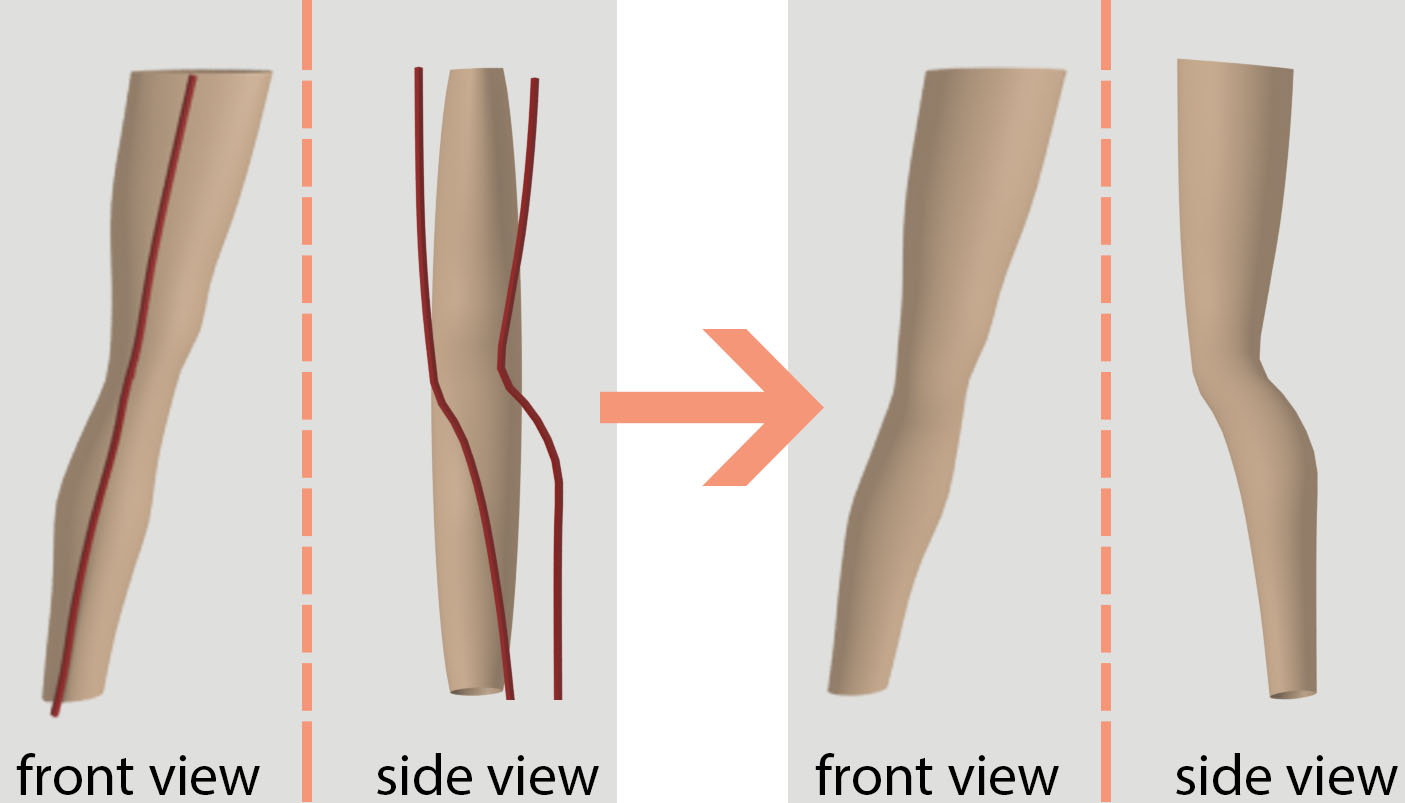
\includegraphics[height=1.3 in]{leg_transformation_free_form.jpg}
    \caption{}
    \label{fig:leg deformed twice}
    \end{subfigure}
    \caption{ODE-driven Sketch-based deformations: (a)the deformation process of an organic shape represented by an ellipsoid and its 2D silhouette contour, and the deformed shape of the ellipsoid, (b) a leg that has been deformed by single-view sketch strokes before, now is further deformed in accordance with free form red-colored curves}
    \label{fig:ODE-driven Sketch-based deformations}
\end{figure}

The aforementioned method was developed in python on the Houdini FX Education Edition 16.5.323 package, and ran on a dual boot Linux PC with 23GB memory and 64 bits Intel(R) Xeon(R) CPU E5-1650 0 @ 3.20GHz CPU. The average time for deforming a cylinder is 0.17 seconds, which ensures a smooth real-time modelling user experience.

\section{Conclusion and future work}\label{Conclusion and future work}
By extending the work described in \cite{li2017bendsketch}, a sketch-based modelling approach has been developed in this paper. It creates base 3D models easily and quickly by first generating silhouette contours of 3D objects, decomposing the generated silhouette contours into parts to obtain the sketch segments of the parts, determining the central lines of parts, automatically placing ellipsoids or straight cylinders by bending the cylinders along the central lines to best align with the sketch segments, scaling the placed ellipsoids to match the sketch segments, minimizing the sum of squired errors between the projected silhouette curves of the placed cylinders and the sketch segments to obtain the optimal radius of the placed cylinders and make the placed cylinder best fit the sketch segments. Furthermore, an ordinary differential equation (ODE)-based deformation algorithm has been developed to deform the placed cylinders so that the projected silhouette curves of the deformed cylinders are exactly the same as the sketch segments.

With our proposed approach, different 3D base models were created from 2D sketches and depicted in Figure \ref{fig:different means to input silhouette}. These created base 3D models indicate that our proposed approach achieves the advantages of: 1) easiness for beginners to use, 2) avoiding heavy manual operations, and 3) high efficiency in creating sketch-based 3D organic models.

\begin{figure}[!htbp]
    \centering
    \begin{subfigure}[p]{.2\linewidth}
    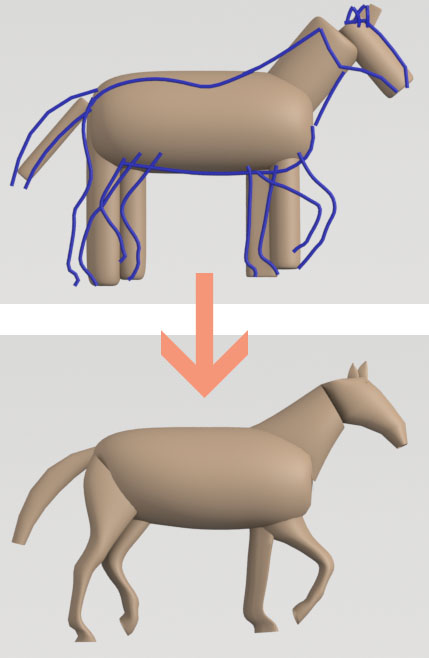
\includegraphics[height=1.3in]{horse_before_and_after.jpg}
    \caption{}
    \label{fig:horse}
    \end{subfigure}
    \begin{subfigure}[p]{.25\linewidth}
    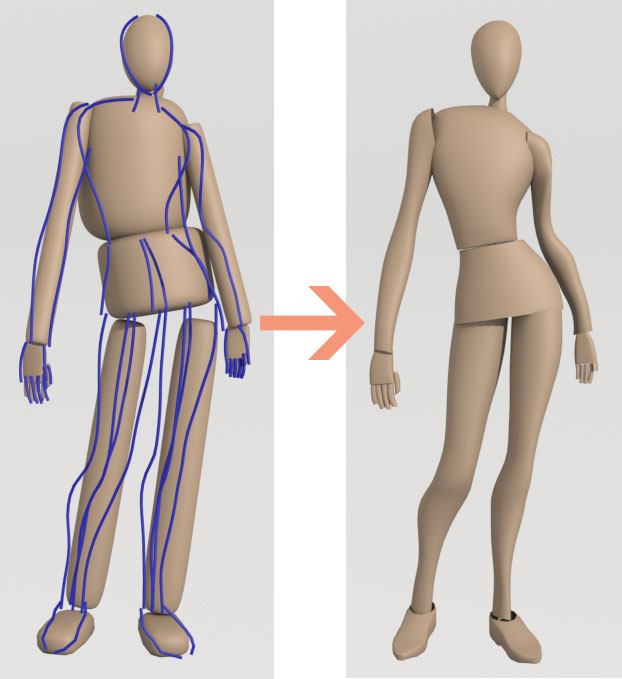
\includegraphics[height=1.3in]{female_primitives_before_and_after_deformation.jpg}
    \caption{}
    \label{fig:female}
    \end{subfigure}
    \begin{subfigure}[p]{.2\linewidth}
    \centering
    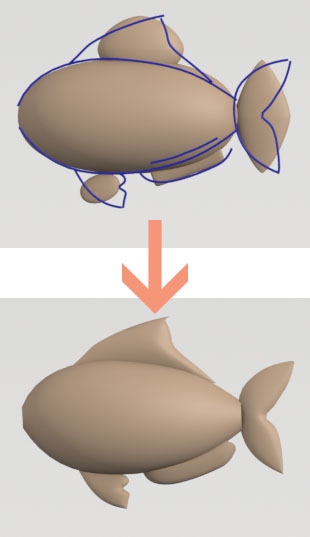
\includegraphics[height=1.3 in]{fish_before_and_after.jpg}
    \caption{}
    \label{fig:fish}
    \end{subfigure}
    \begin{subfigure}[p]{.2\linewidth}
    \centering
    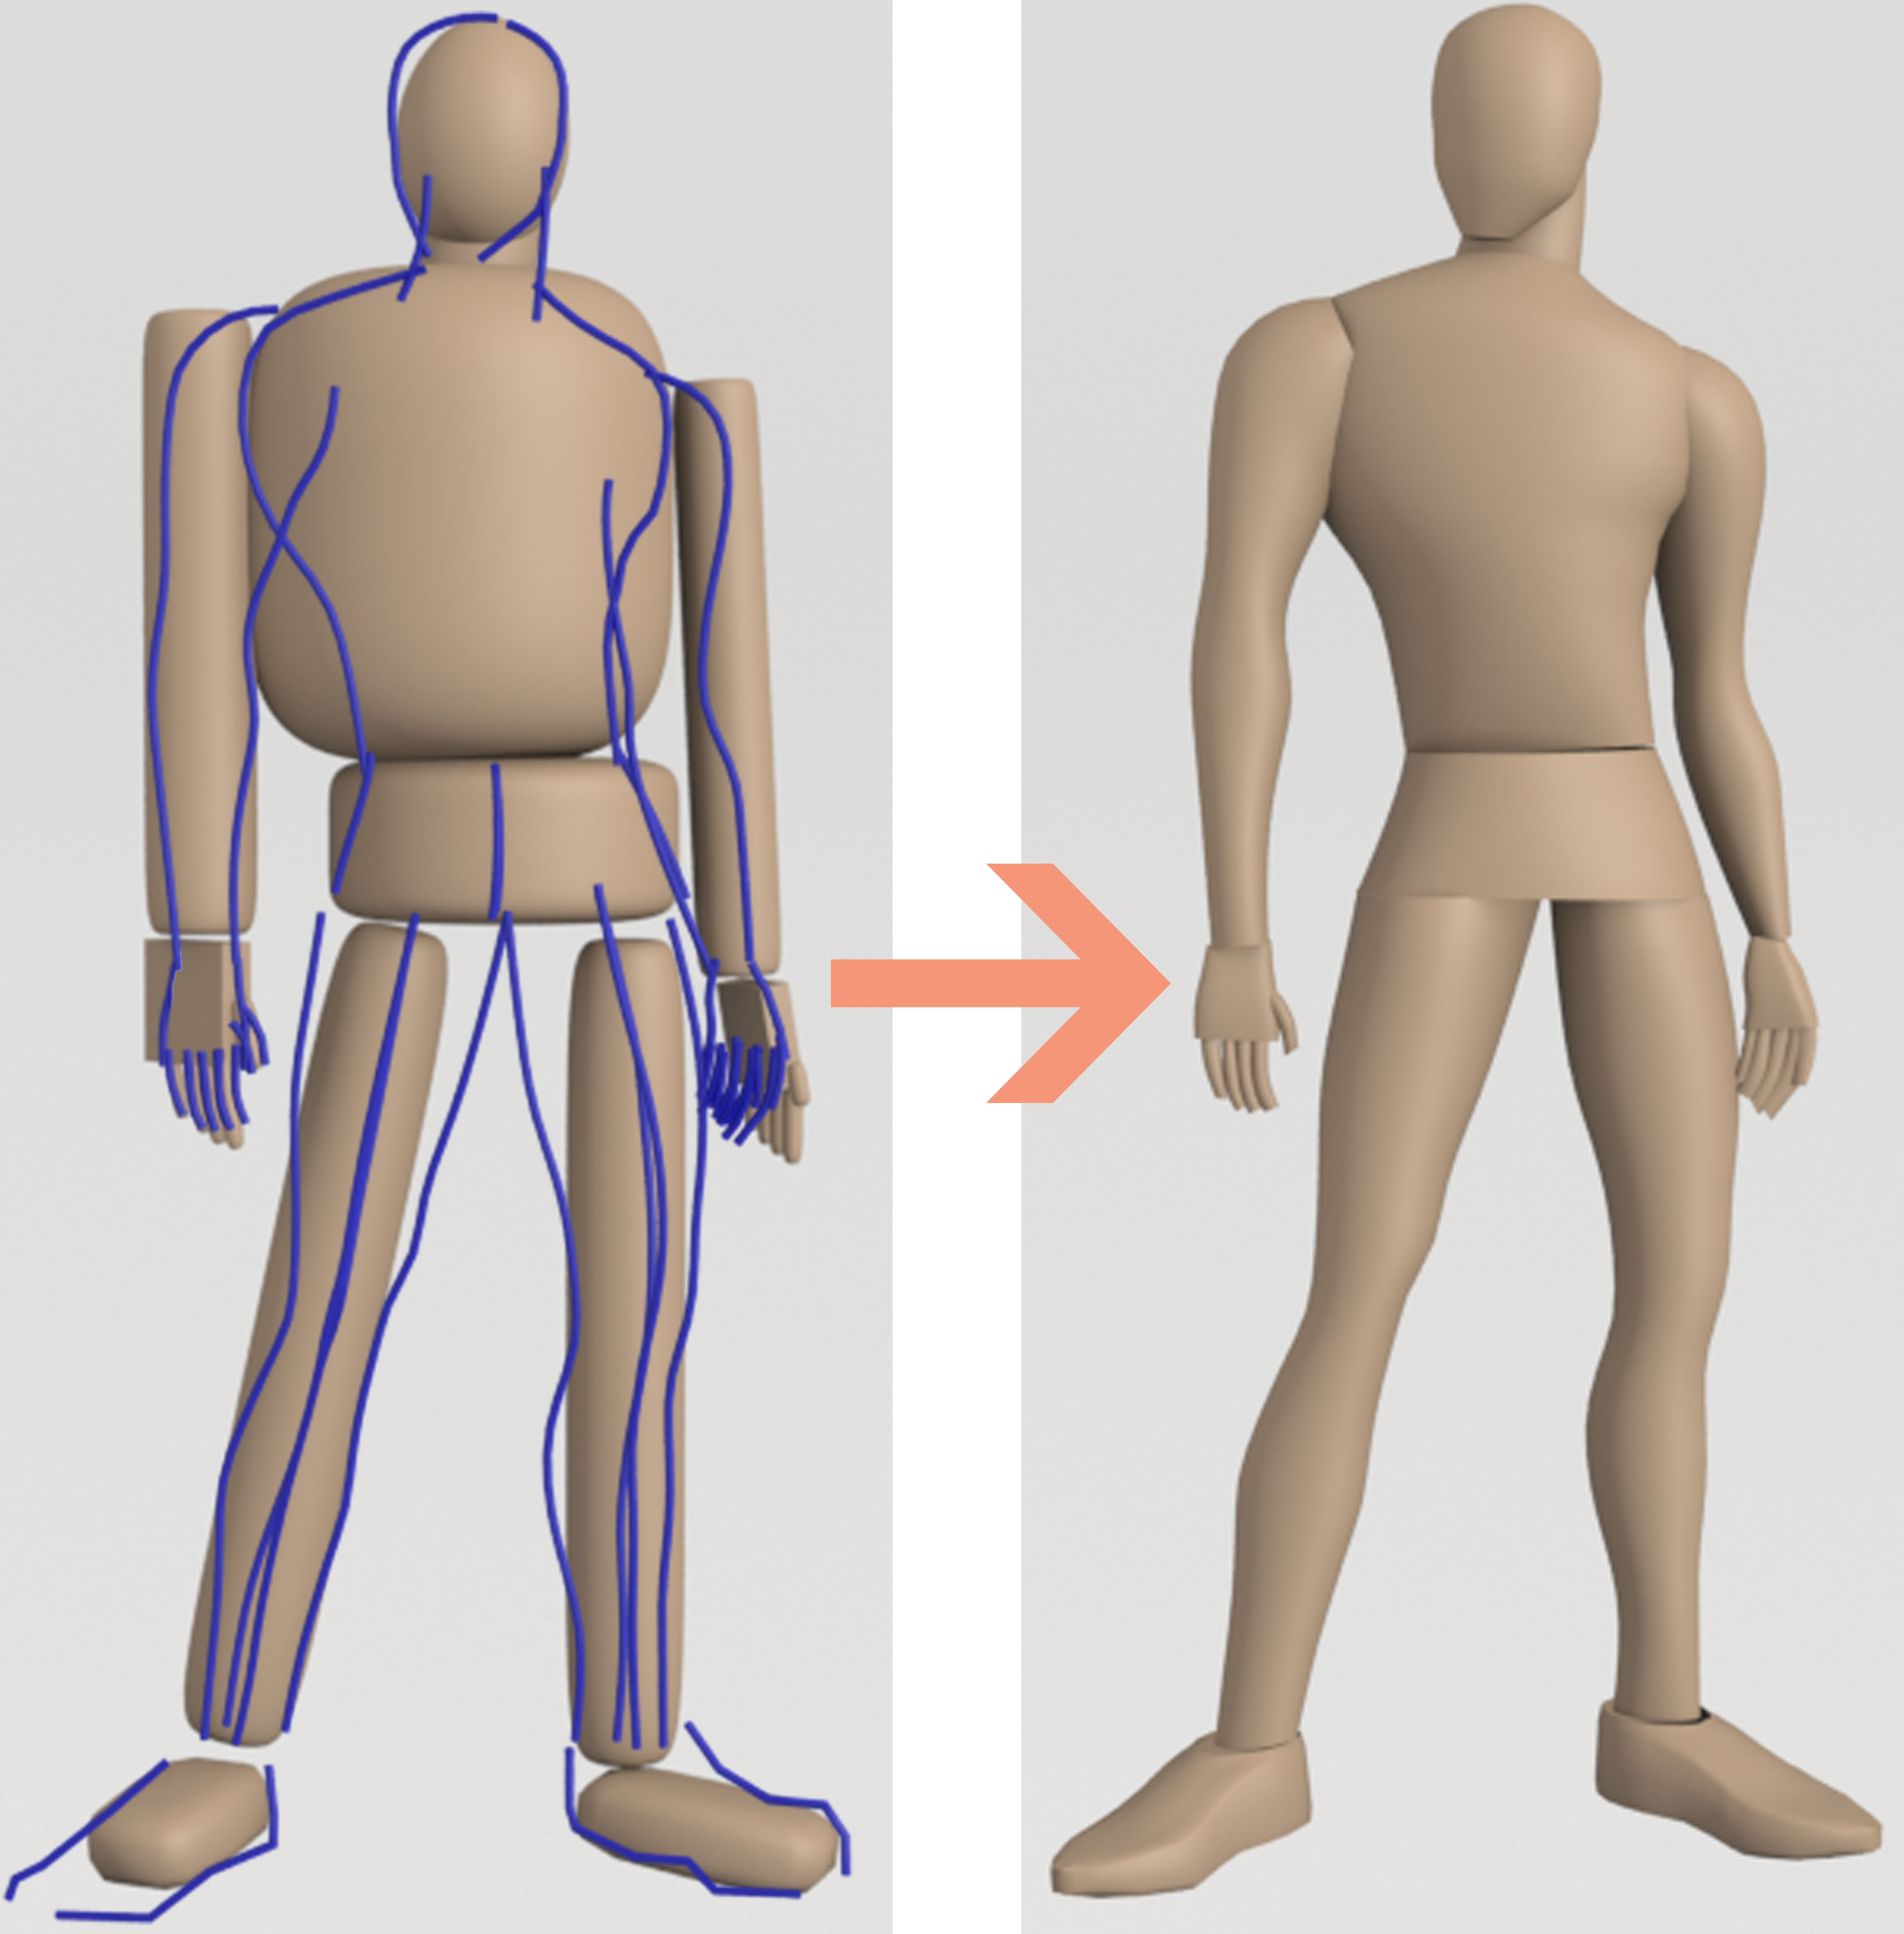
\includegraphics[height=1.3 in]{male_primitive_before_and_after.jpg}
    \caption{}
    \label{fig:male}
    \end{subfigure}
    \caption{Examples of the primitive deformation method}
    \label{fig:different means to input silhouette}
\end{figure}

Up to now, various sketch-based 3D modelling approaches can only create rough 3D models. How to develop new sketch-based modelling approaches to create detailed and realistic 3D models still has a long way to go. The approach proposed in this paper tackles how to create rough 3D base models easily and quickly. In our following work, we will further investigate various sketch-guided and ODE-based deformation methods to obtain detailed deformations and create local 3D shapes for more realistic sketch-based 3D modelling. 

\section{Acknowledgements}\label{Acknowledgements}
This research is supported by the PDE-GIR project which has received funding from the European Unions Horizon 2020 research and innovation programme under the Marie Skodowska-Curie grant agreement No 778035, and Innovate UK (Knowledge Transfer Partnerships Ref: KTP010860).

%
% ---- Bibliography ----
%
% BibTeX users should specify bibliography style 'splncs04'.
% References will then be sorted and formatted in the correct style.
%
 \bibliographystyle{splncs04}
 \bibliography{reference.bib}
%

\end{document}

